\documentclass[letterpaper, 10 pt, conference]{ieeeconf}

\overrideIEEEmargins
\usepackage[pdftex]{graphicx}

\title{\LARGE \bf Deep Learning for Anomaly Detection in Networks and Images}
\author{Andy Malinsky}% <-this % stops a space

\begin{document}
\maketitle
\thispagestyle{empty}
\pagestyle{empty}

\begin{abstract}
Deep learning techniques have had a widespread impact on methods of anomaly detection in various domains. Within cybersecurity, the importance of detecting outsider threats and uncommon patterns in data plays a crucial role in preserving security in systems. In this light, deep learning techniques have been applied to network intrusion detection systems. This paper surveys some of the recent applications of deep learning to anomaly detection in cybersecurity along with some general applications to other areas.
\end{abstract}
\hfill

\section{INTRODUCTION}
Computer security still exhibits a major area of concern as the threat of cyber attacks still persists. Figure \ref{incident_chart} displays the number of security incidents over a recent five year time period. Network security still exhibits a major area of concern as the threat of cyber attacks still persists. One technique of combating cyber threats is through anomaly detection. Such techniques model the normal network and system behavior, and use this information to identify anomalies, or deviations, from normal behavior \cite{c1}. One example of an anomaly is an unusual network traffic pattern, because it could mean that a computer may have been compromised and data has been transmitted to suspicious locations \cite{c7}. Many have turned to approaches from deep learning for constructing anomaly detection systems. In general terms, deep learning is a subset of machine learning that involves the use of artificial neural networks with multiple layers to solve problems of optimization or detection. This paper will review some of the deep learning approaches to anomaly detection, focusing on network security and then extending to other applicable areas.

\begin{figure}[ht!] %!t
\centering
\hspace*{-5.1cm}
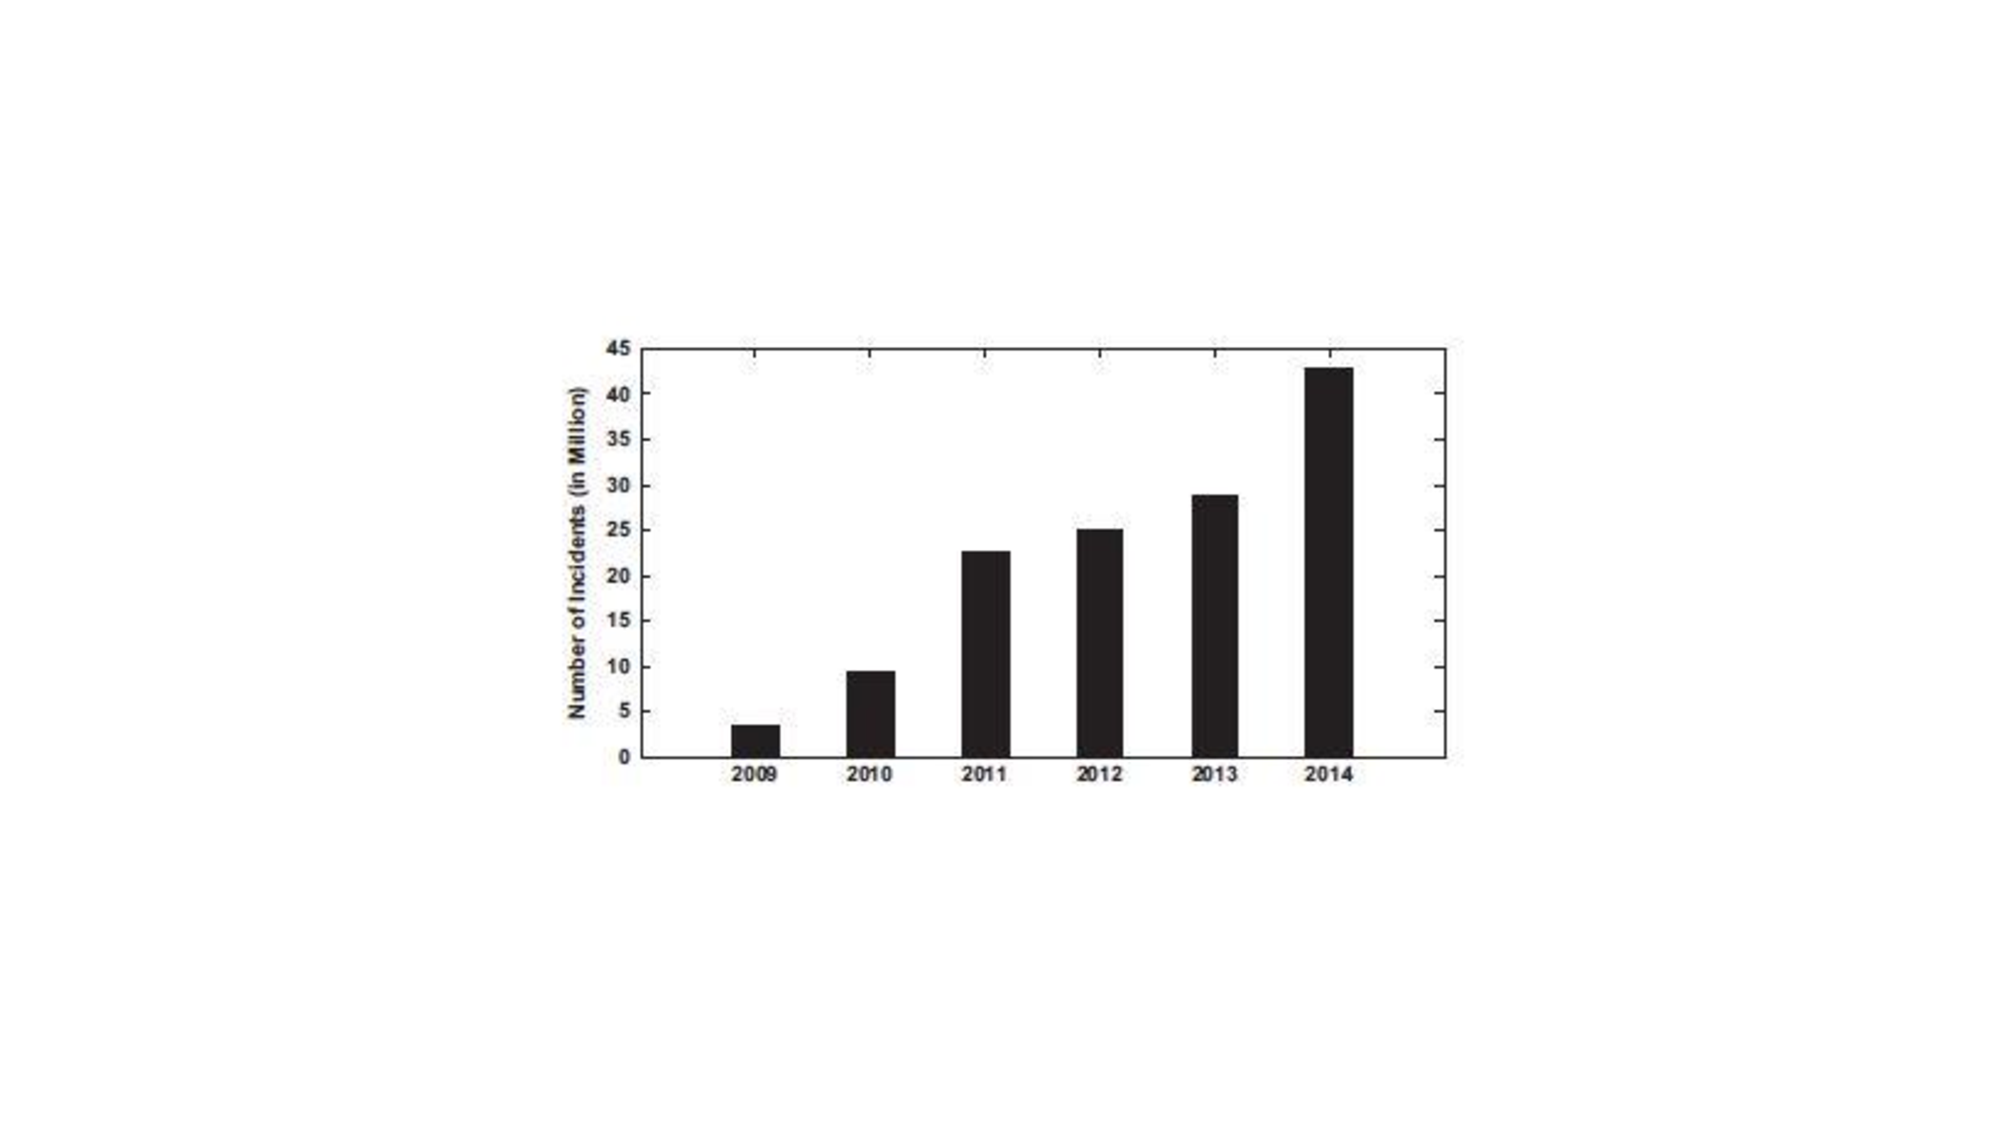
\includegraphics[height=3in, trim={0 0 0 5cm}, clip]{incident_chart.pdf}
\vspace*{-35mm}
\caption{Depicted is the growth of security incidents from 2009 to 2014 by The Global State of Information Security Survey 2015 \cite{c7, c11}.}
\label{incident_chart}
\end{figure}


\hfill
\section{LITERATURE REVIEW}

\subsection{Self-taught Learning}
One deep learning approach to network security is the use of Self-taught Learning (STL) \cite{c2}. This is an approach geared toward improving current Network Intrusion Detection Systems (NIDS), as there are some challenges to be addressed. When dealing with anomaly detection the system has to be able to identify certain threats when they may present themselves. However, new threats are constantly arising so selecting the proper features as anomalies should not just apply to a single type of attack. Also, new labeled datasets from real network traffic may be hard to collect from administrators. Proposed is STL, which consists of a two stage classification process. First it goes through a large set of unlabeled data and learns a stable feature representation. Second, it applies the representation to labeled data which is then used for classification. This process can be seen in Figure \ref{self_learning_figure}. The STL NIDS was tested on the NSL-KDD, a standard dataset for network intrusion, to evaluate anomaly detection accuracy. The proposed STL NIDS performed very well against previously implemented NIDS.

\begin{figure}[ht!] %!t
\centering
\hspace*{0.4cm}
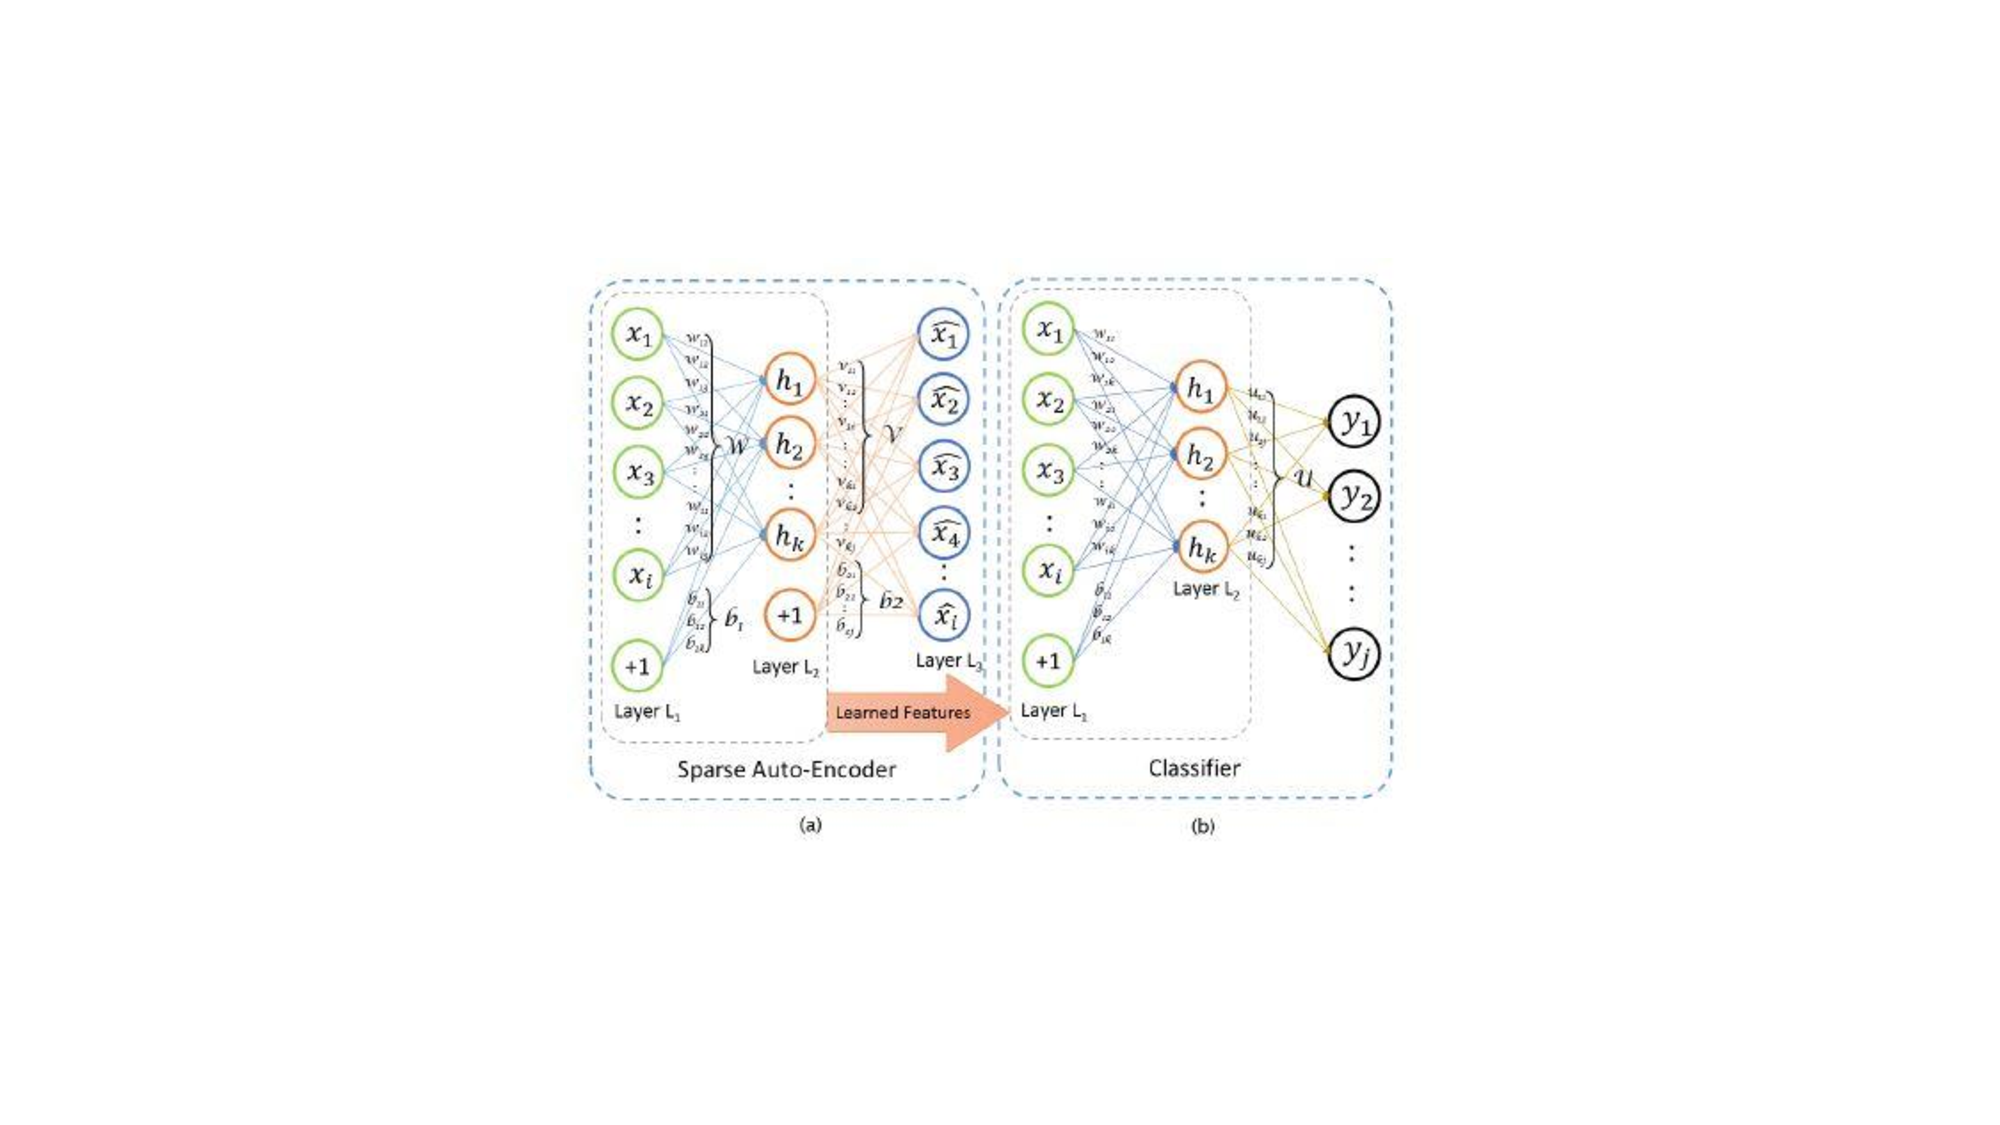
\includegraphics[height=3in, trim={10cm 0 10cm 4cm}, clip]{self_learning_figure.pdf}
\vspace*{-25mm}
\caption{The STL process begins with "Unsupervised Feature Learning" on unlabeled data. A sparse autoencoder was used for feature learning. This neural network first utilized the backpropagation algorithm to minimize the cost function, and then used soft-max regression for the classification task \cite{c2}.}
\label{self_learning_figure}
\end{figure}

\hfill
\subsection{Simple Deep Neural Network}
Deep learning has also been applied to network intrusion detection in software defined networking (SDN) \cite{c3}. The SDN architecture is directly programmable, agile, centrally managed, programmatically configured, and implemented through open standards \cite{c12}. A Deep Neural Network (DNN) is applied to the NIDS model in an SDN context. 

\begin{figure}[ht!] %!t
\centering
\hspace*{0.4cm}
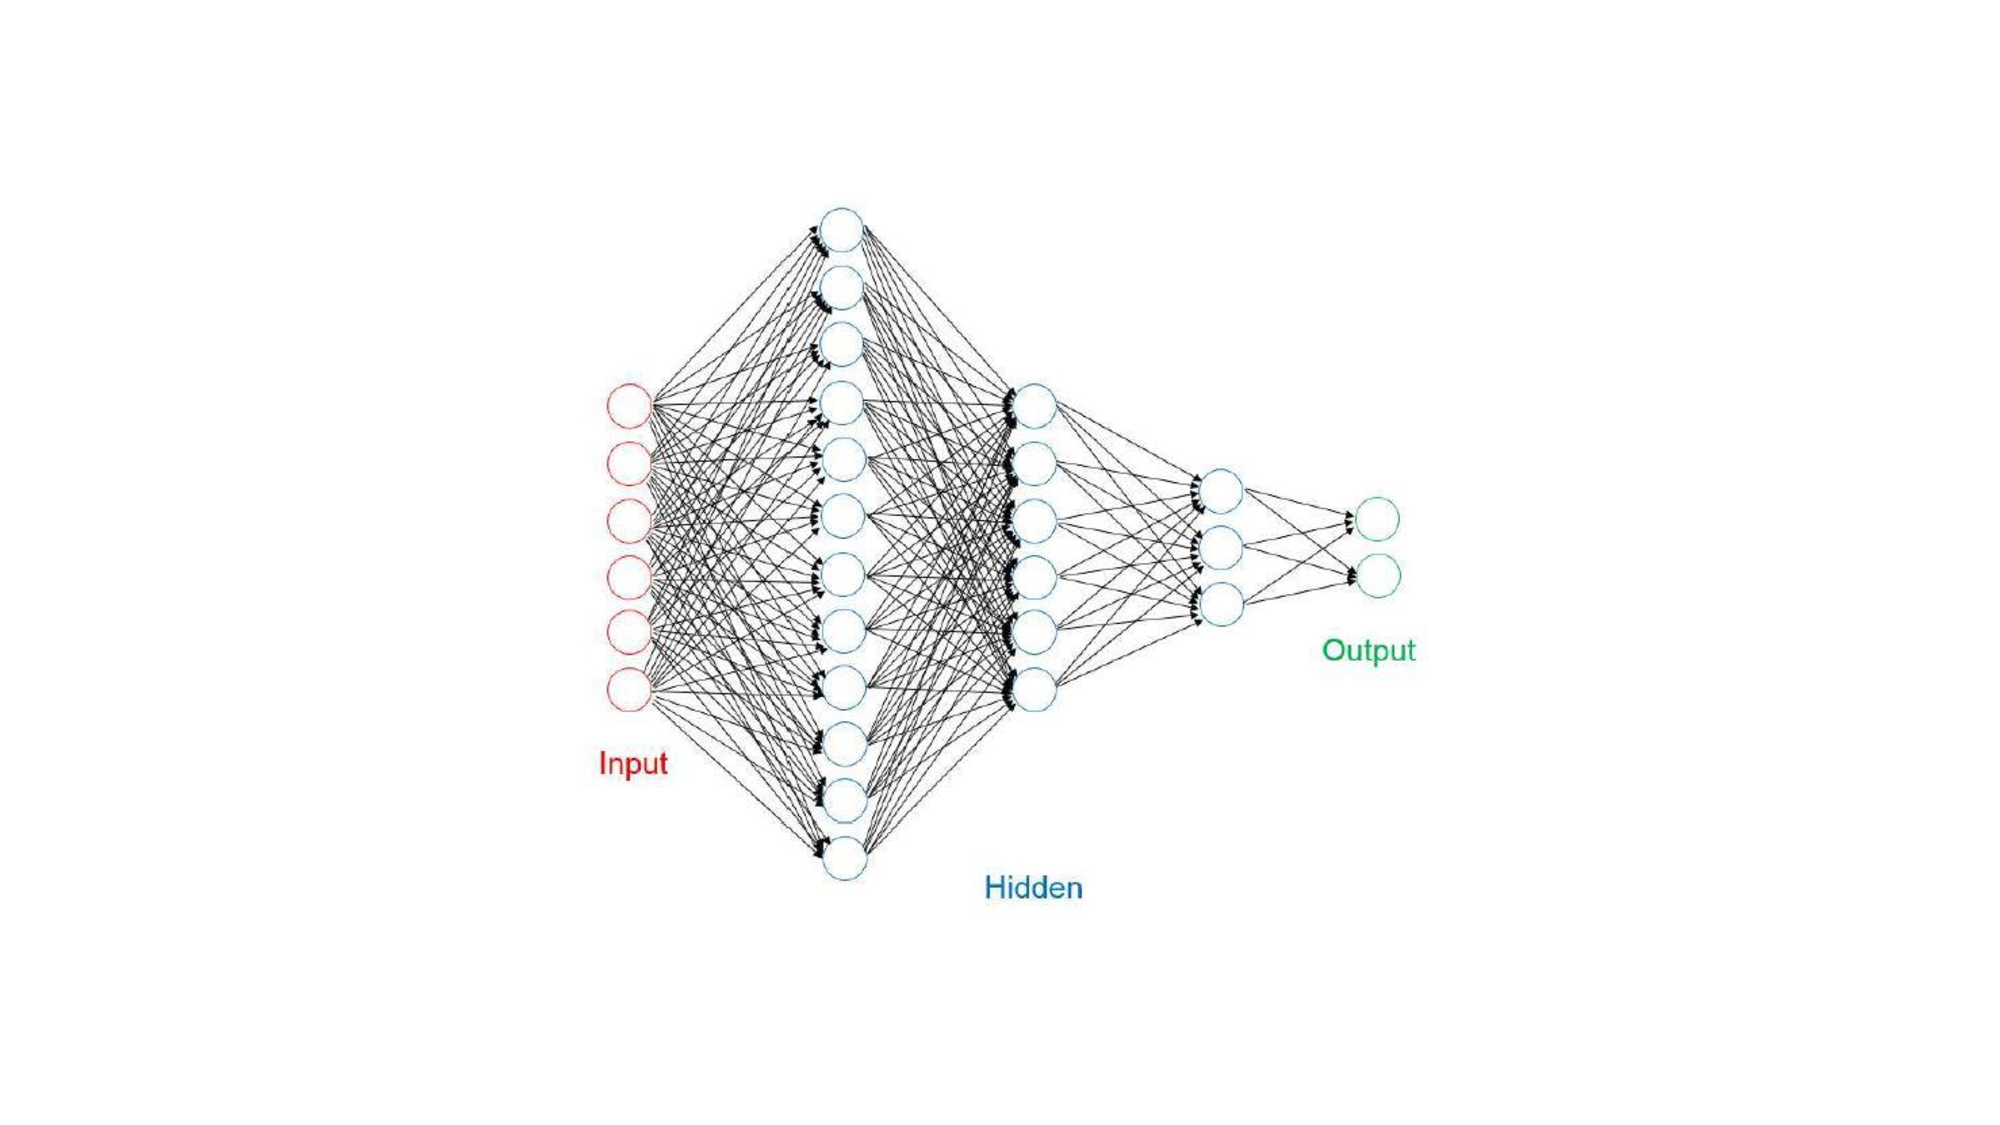
\includegraphics[height=3in, trim={10cm 0 10cm 4cm}, clip]{deep_net_figure.pdf}
\vspace*{-15mm}
\caption{The STL process begins with "Unsupervised Feature Learning" on unlabeled data. A sparse autoencoder was used for feature learning. This neural network first utilized the backpropagation algorithm to minimize the cost function, and then used soft-max regression for the classification task \cite{c3}.}
\label{deep_net_figure}
\end{figure}

The proposed Deep Neural Network approach yielded a higher accuracy rate when compared to other approaches including the Naive Bayes, Support Vector Machine, and Decision Tree algorithms. The deep neural newtork is able to generalize features of network traffic and attain an abstract level of understanding. There is still room for further development, but deep learning anomaly detection based systems has proven potential.

\hfill
\subsection{Long Short Term Memory}
Another deep learning approach to an Intrusion Detection System (IDS) model is the use of a Long Short Term Memory (LSTM) architecture \cite{c4}. In this case, a LSTM was applied to a Recurrent Neural Network (RNN) and tested against the KDD Cup 1999 dataset.

\begin{figure}[ht!] %!t
\centering
\hspace*{0.4cm}
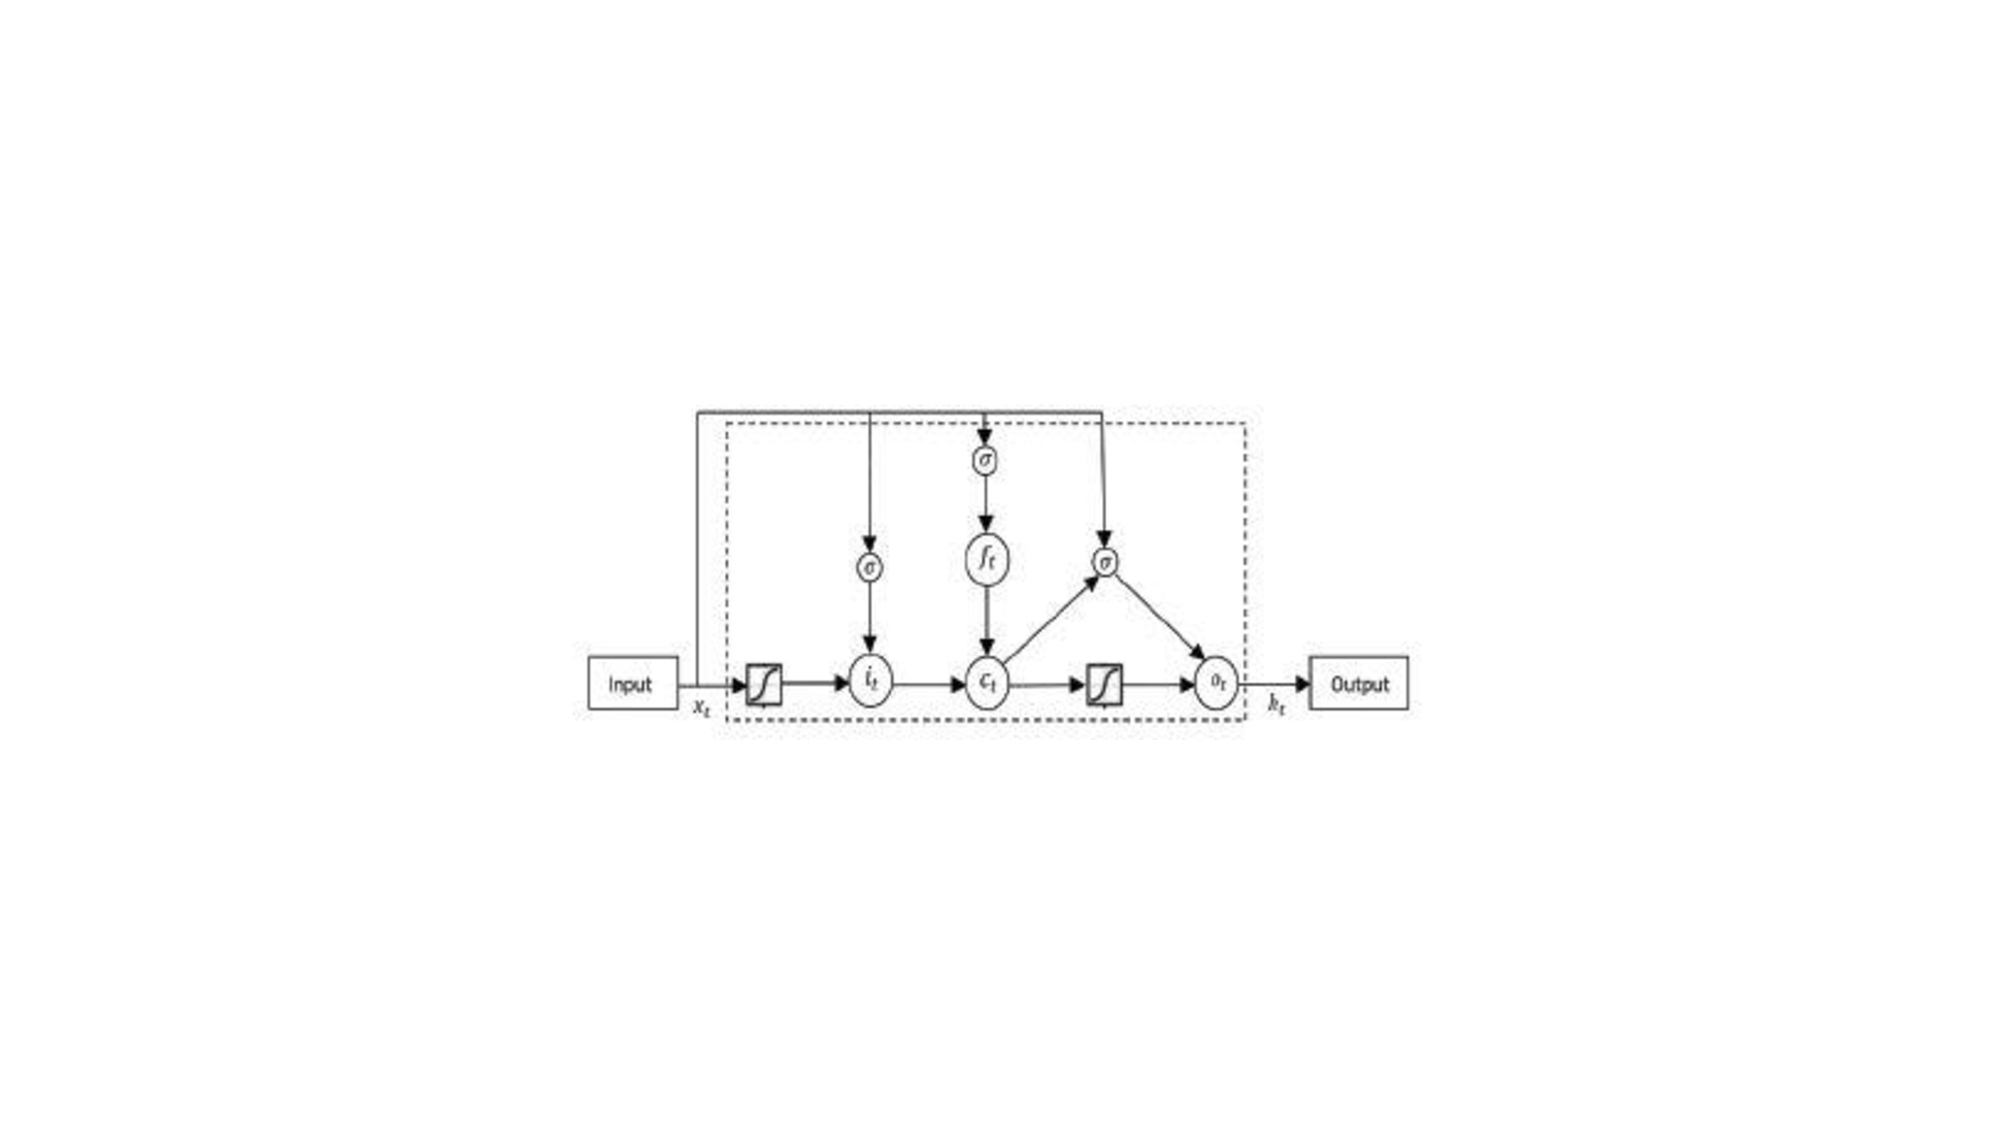
\includegraphics[height=3in, trim={10cm 0 10cm 4cm}, clip]{lstm_figure.pdf}
\vspace*{-25mm}
\caption{The LSTM cell, as depicted in the figure, consists of three gates: input, forget, and output \cite{c4}. The overall function of the cell is to solve the vanishing and exploding gradient problems by controlling the information flow.}
\label{lstm_figure}
\end{figure}

An IDS classifier was implemented and evaluated based on a LSTM-RNN model. It was found that this model was able to detect attacks with a greater detection rate accuracy when compared to other classifier algorithms. However, there is still room for improvement in reducing the False Alarm Rate, or the ratio of misclassified normal instances.

\hfill
\subsection{Online Unsupervised Learning}
Deep learning techniques have also been applied to structured cybersecurity data streams \cite{c5}. One area of data analysis prevalent in cybersecurity is log analysis. The sheer volume of streaming data that can be found within a single system log calls for an automated approach for detecting anomalies. Proposed is an online unsupervised deep learning approach. This technique is able to detect network anomalies in real time from system logs. Similarly to the aforementioned paper, this model utilizes a DNN and RNN model that uses the LSTM architecture. It was tested against the CERT Insider Threat Dataset v6.2. This attempt is different as, instead of training in individual or batches of sequences, the RNN trains on multiple user sequences concurrently. Results showed that the proposed DNN and LSTM models outperformed three standard anomaly detection techniques: Isolation Forest, Support Vector Machines, and Principal Component Analysis. Room for further development could be implementing a more generalized approach than focusing on insider threat patterns, as this experiment had done.

\hfill
\subsection{Recurrent Neural Networks}
A slightly different deep learning approach to an IDS involves a standard RNN model \cite{c6}. Instead of having a LSTM cell or a separate DNN manipulate parameters, the RNN architecture just utilizes standard recurrent hidden layers. RNN have a directional loop that can apply previous information to the current output. The current output is related to the preceding output with connections between the nodes of the respective hidden layers.

\begin{figure}[ht!] %!t
\centering
\hspace*{0.4cm}
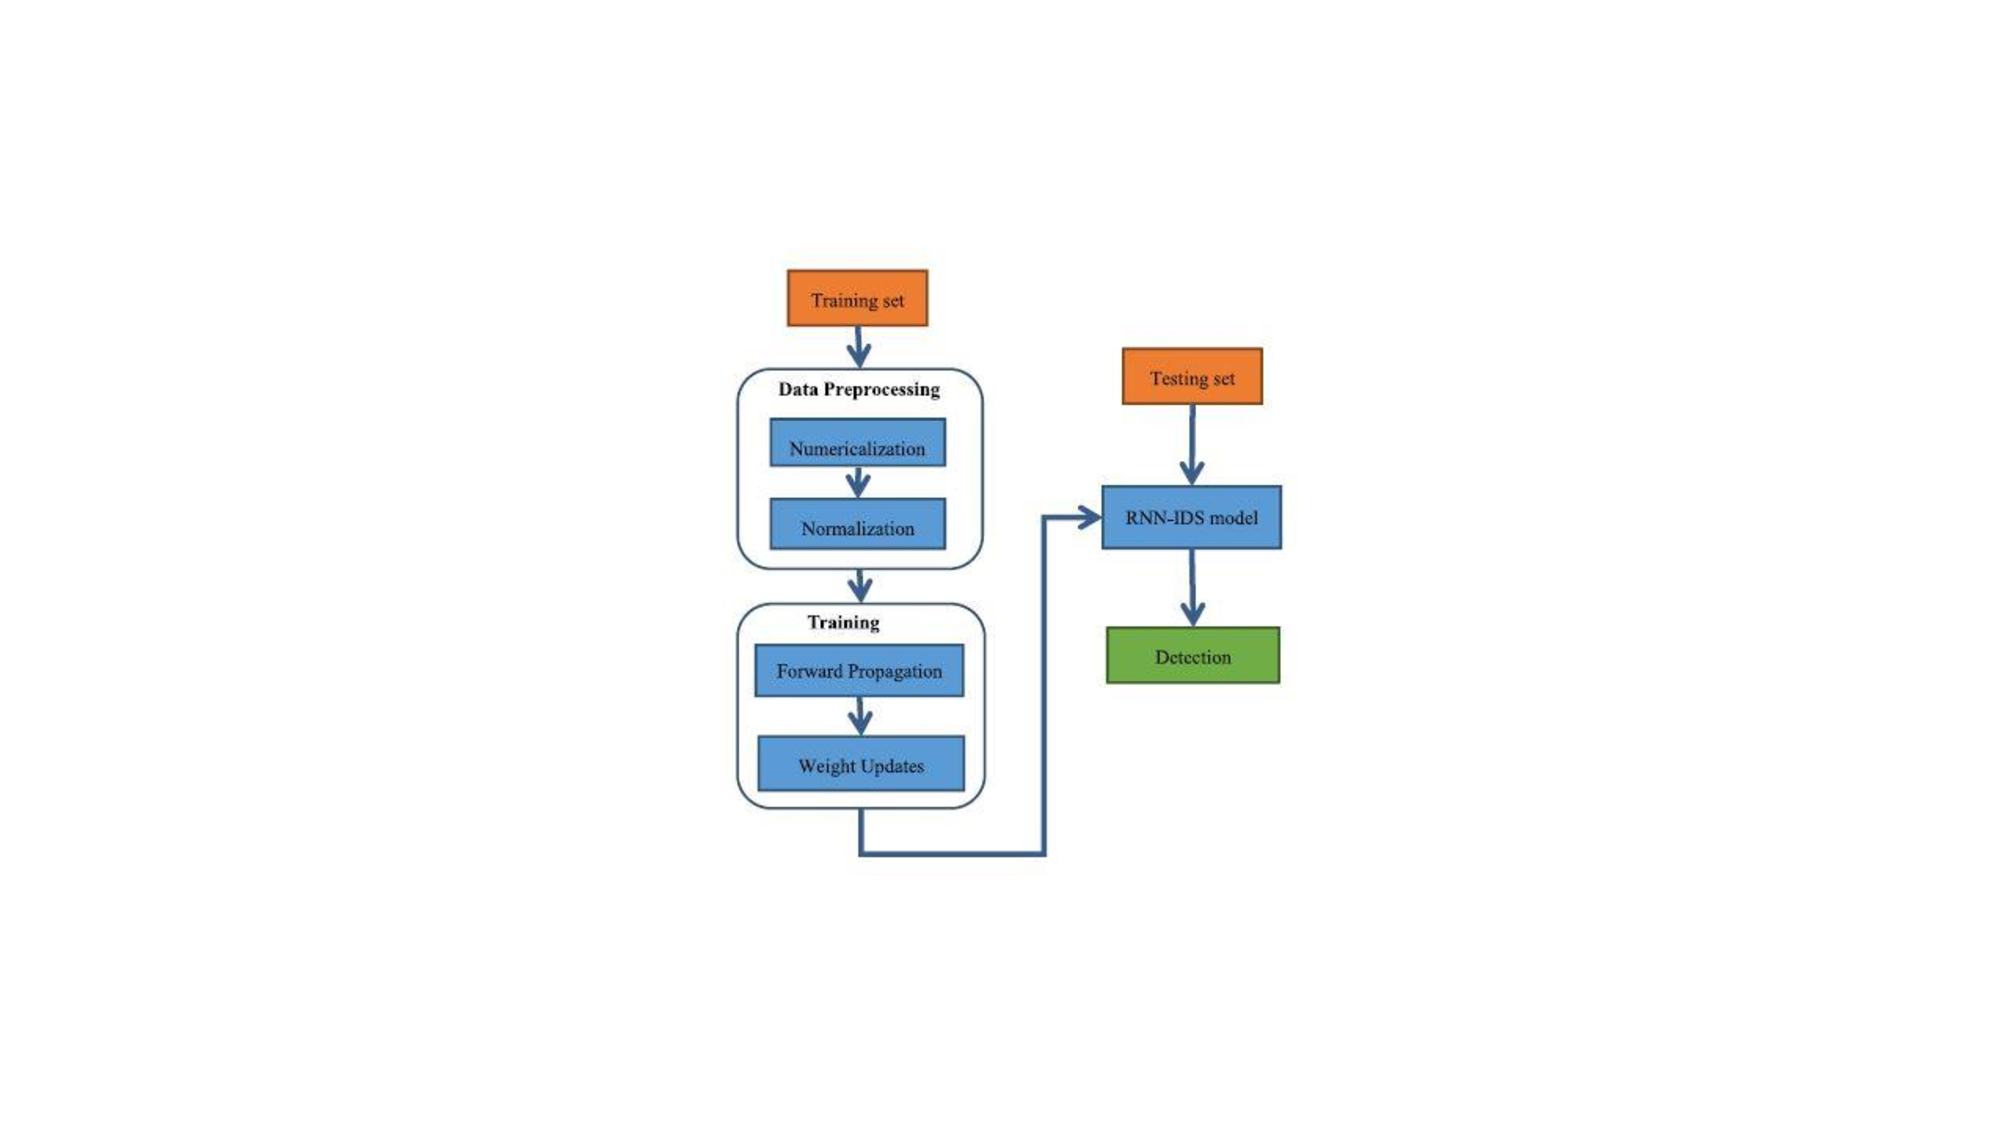
\includegraphics[height=3in, trim={10cm 0 10cm 4cm}, clip]{rnn_figure.pdf}
\vspace*{-25mm}
\caption{A block diagram of the proposed RNN-IDS \cite{c6}. Depicted are the steps involved in the implementation of the RNN-IDS model.}
\label{rnn_figure}
\end{figure}

The model was tested against the NSL-KDD dataset, and yielded high accuracy in both binary and multiclass classification. It also outperformed other classification methods such as the J48, Naive Bayes, and random forest algorithms. An aspect for improvement is in reducing training time through GPU acceleration.

\subsection{Convolutional Neural Networks}
One deep learning approach to anomaly detection involves the use of Convolutional Neural Networks (CNN) \cite{c8}. Utilized are CNNs for detecting abnormal behavior in crowded scenes through recorded video. This is related to security as this approach is applicable to surveillance cameras. Rare shapes or motions are learned from training samples that teach normal behaviors of regions. CNNs are useful for image classification \cite{c13}, object detection \cite{c14}, or activity recognition \cite{c15, c8}. This proposed CNN model represents a video using a set of regional features. Throughout the training process, it classifies regions as ``suspicious'' or not and extracts features that would classify as anomalies. This paper utilized Fully Convolutional Networks (FCNs) for anomaly detection and was evaluated on the UCSD and Subway benchmarks. The proposed method was shown to outperform existing methods with respect to processing speed.

CNNs have also been applied to fault detection \cite{c9}. Monitoring rotating machinery is an important task for maintaining a productive environment. One method of condition monitoring for rotating machines is vibration analysis. The feature-learning CNN was tested against and compared to a feature-engineering approach using manual features and a random forest classifier. Results yielded a stronger accuracy for the CNN approach, greater by six percent. This shows that less initial domain expertise is required for feature learning. Room for future development includes the reduction of misclassifications.

\hfill
\section{OPEN ISSUES AND FUTURE DIRECTIONS}
Anomaly detection is a major area for cybersecurity. Protecting network information is vitally important. Deep learning techniques have been employed as a means of offering solutions for various Intrusion Detection Systems. Current challenges include reducing the training time for feature learning and reducing the false detection rate made with misclassifications. Also, there is room for more development in the application of the Long Short Term Memory method for Recurrent Neural Network architectures. More research into the combination and implementation of Deep Neural Networks with various models may yield more promising results for future work in the area of anomaly detection. 

\addtolength{\textheight}{-12cm}

\hfill
\begin{thebibliography}{99}

\bibitem{c1} Buczak, A. L., \& Guven, E. (2016). A survey of data mining and machine learning methods for cyber security intrusion detection. IEEE Communications Surveys \& Tutorials, 18(2), 1153-1176.
\bibitem{c2} Javaid, A., Niyaz, Q., Sun, W., \& Alam, M. (2016, May). A deep learning approach for network intrusion detection system. In Proceedings of the 9th EAI International Conference on Bio-inspired Information and Communications Technologies (formerly BIONETICS) (pp. 21-26). ICST (Institute for Computer Sciences, Social-Informatics and Telecommunications Engineering).
\bibitem{c3} Tang, T. A., Mhamdi, L., McLernon, D., Zaidi, S. A. R., \& Ghogho, M. (2016, October). Deep learning approach for network intrusion detection in software defined networking. In 2016 International Conference on Wireless Networks and Mobile Communications (WINCOM) (pp. 258-263). IEEE.
\bibitem{c4} Kim, J., Kim, J., Thu, H. L. T., \& Kim, H. (2016, February). Long short term memory recurrent neural network classifier for intrusion detection. In 2016 International Conference on Platform Technology and Service (PlatCon) (pp. 1-5). IEEE.
\bibitem{c5} Tuor, A., Kaplan, S., Hutchinson, B., Nichols, N., \& Robinson, S. (2017, March). Deep learning for unsupervised insider threat detection in structured cybersecurity data streams. In Workshops at the Thirty-First AAAI Conference on Artificial Intelligence.
\bibitem{c6} Yin, C., Zhu, Y., Fei, J., \& He, X. (2017). A deep learning approach for intrusion detection using recurrent neural networks. Ieee Access, 5, 21954-21961.
\bibitem{c7} Ahmed, M., Mahmood, A. N., \& Hu, J. (2016). A survey of network anomaly detection techniques. Journal of Network and Computer Applications, 60, 19-31.
\bibitem{c8} Sabokrou, M., Fayyaz, M., Fathy, M., Moayed, Z., \& Klette, R. (2018). Deep-anomaly: Fully convolutional neural network for fast anomaly detection in crowded scenes. Computer Vision and Image Understanding, 172, 88-97.
\bibitem{c9} Janssens, O., Slavkovikj, V., Vervisch, B., Stockman, K., Loccufier, M., Verstockt, S., ... \& Van Hoecke, S. (2016). Convolutional neural network based fault detection for rotating machinery. Journal of Sound and Vibration, 377, 331-345.
\bibitem{c10} Schlegl, T., Seeböck, P., Waldstein, S. M., Schmidt-Erfurth, U., \& Langs, G. (2017, June). Unsupervised anomaly detection with generative adversarial networks to guide marker discovery. In International Conference on Information Processing in Medical Imaging (pp. 146-157). Springer, Cham.
\bibitem{c11} The Global State of Information Security Survey 2015. http://www.pwc.com.
\bibitem{c12} “Software Defined Networking Definition,” Available:
https://www.opennetworking.org/sdn-resources/sdn-definition, [Accessed 22 Apr. 2019].
\bibitem{c13} Krizhevsky, A., Sutskever, I., Hinton, G.E., 2012. ImageNet classification with deep
convolutional neural networks. Adv. Neural Inf. Process. Syst. 1097–1105.
\bibitem{c14} Girshick, R., Donahue, J., Darrell, T., Malik, J., 2014. Rich feature hierarchies for accurate
object detection and semantic segmentation. Computer Vision Pattern Recognition.
pp. 580–587.
\bibitem{c15} Simonyan, K., Zisserman, A.,. Two-stream convolutional networks for action recognition
in videos. CoRR, arXiv:1406.2199.

\end{thebibliography}
\end{document}